\documentclass[micros_g1_main.tex]{subfiles}
\begin{document}

\section{Abreviaciones}

Incluímos la siguientes abreviaciones para agilizar la lectura del informe:

	\begin{itemize}
		\item KRM: Kinetis K64 SubFamily Reference Manual.
		\item KD: Kinetis K64F SubFamily Datasheet.
	\end{itemize}
	
\section{Ejercicio 1}


\subsection{Ítem a}
El puerto PTA12 se encuentra en el pin 42.\par
Este dato se encuentra en el KRM, en la sección 10.3.1, sección de pinout, tanto en las tablas de la sección 10.3.1. como en el diagrama de pinout (figura 10.5) del 100 LQFP. \par
A su vez, el mismo se encuentra en la KD, en la sección 5.1, sección de pinout.

\subsection{Ítem b}
Al inspeccionar la hoja de datos del microontrolador, se encuentra cuántos y cuáles son los pines que tienen conversores AD. El fabricante nos proporciona una lista con las interfaces analógicas disponibles, es decir, que no están reservados para el microcontrolador. El microcontrolador cuenta con 11 pines disponibles que admiten entrada analógica, se muestran en la Figura \ref{fig:adc_interfaces}

\begin{figure}[ht]
\centering
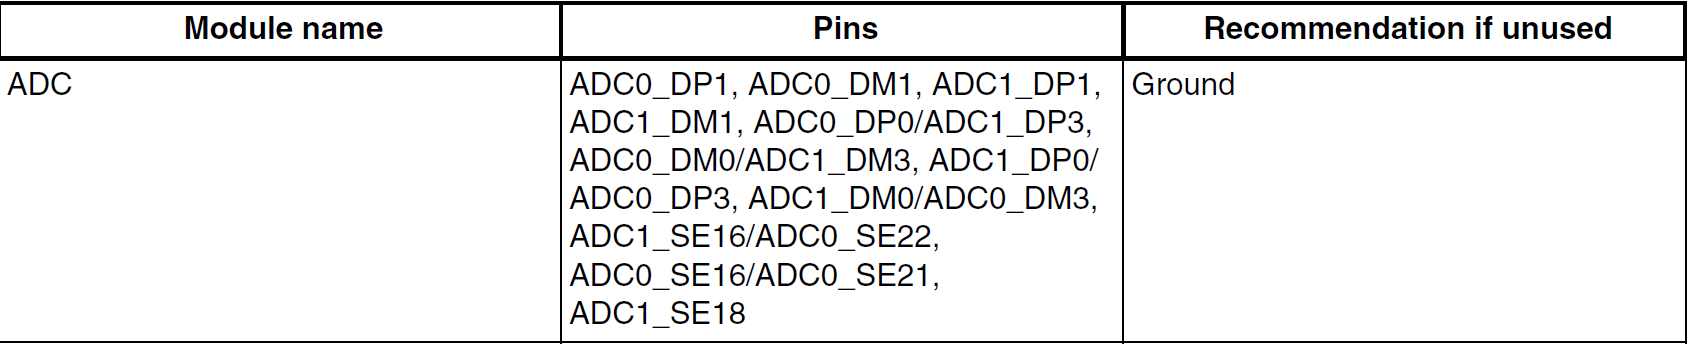
\includegraphics[scale=0.7]{images/adc_interfaces.png}
\caption{Lista de interfaces ADC}
\label{fig:adc_interfaces}
\end{figure}

\subsection{Ítem c}

En este modelo de MCU se encuentran 10 pines disponibles para el puerto PTE, los pines 1 a 7 y 31 a 33. Esto se obtiene tanto de la KD en la sección 5.1, como del KRM en la sección 10.3.1 y de la figura 10.5 ya mencionadas en el ítem a.

\subsection{Ítem d}
VDD es la tensión de alimentación digital utilizada, cuyo rango puede variar entre [-0.3; 3.8](V).\par
El rango para que la tensión de high VIH sea considerada como tal, depende de la tensión VDD, de manera tal que si VDD$\epsilon$ [2.7; 3.6](V), entonces la tensión VIH $\epsilon$ [0.7$\cdot$ VDD; $V_{max}$](V), donde $V_{max}$ es la tensión máxima que admite el pin digital. Al mismo tiempo, si VDD $\epsilon$ [1.7; 2.7](V), entonces VIH $\epsilon$ [0.75$\cdot$ VDD; $V_{max}$](V)\par
En la sección 1.4 del KD, Voltage and current operating ratings, se encuentra el rango de entrada y salida digital para los pines de entrada y salida: [-0.3; 5.5](V) para aquellos pines que no son el RESET, XTAL y EXTAL. Para estos últimos pines el rango es de [-0.3; VDD+0.3] (V). Es por esto que para los pines que no son el RESET, XTAL y EXTAL, los mismos aceptan una tensión de 5(V). Por otro lado, los pines RESET, XTAL y EXTAL NO aceptan una tensión de 5(V).\par

\subsection{Ítem e}
En la sección 1.4 de la KD, se observa que la máxima corriente que puede entregar un pin cualquiera es 25mA.


\end{document}
